\documentclass[journal,12pt,twocolumn]{IEEEtran}
%
\usepackage{setspace}
\usepackage{gensymb}
%\doublespacing
\singlespacing

\usepackage[cmex10]{amsmath}
\usepackage{amsthm}
%\usepackage{iithtlc}
\usepackage{mathrsfs}
\usepackage{txfonts}
\usepackage{stfloats}
\usepackage{bm}
\usepackage{cite}
\usepackage{cases}
\usepackage{subfig}
%\usepackage{xtab}
\usepackage{longtable}
\usepackage{multirow}
%\usepackage{algorithm}
%\usepackage{algpseudocode}
\usepackage{enumitem}
\usepackage{mathtools}
\usepackage{steinmetz}
\usepackage{tikz}
\usepackage{circuitikz}
\usepackage{verbatim}
\usepackage{tfrupee}
\usepackage[breaklinks=true]{hyperref}
%\usepackage{stmaryrd}
\usepackage{tkz-euclide} % loads  TikZ and tkz-base
%\usetkzobj{all}
\usetikzlibrary{calc,math}
\usepackage{listings}
    \usepackage{color}                                            %%
    \usepackage{array}                                            %%
    \usepackage{longtable}                                        %%
    \usepackage{calc}                                             %%
    \usepackage{multirow}                                         %%
    \usepackage{hhline}                                           %%
    \usepackage{ifthen}                                           %%
  %optionally (for landscape tables embedded in another document): %%
    \usepackage{lscape}     
\usepackage{multicol}
\usepackage{chngcntr}
%\usepackage{enumerate}

%\usepackage{wasysym}
%\newcounter{MYtempeqncnt}
\DeclareMathOperator*{\Res}{Res}
%\renewcommand{\baselinestretch}{2}
\renewcommand\thesection{\arabic{section}}
\renewcommand\thesubsection{\thesection.\arabic{subsection}}
\renewcommand\thesubsubsection{\thesubsection.\arabic{subsubsection}}

\renewcommand\thesectiondis{\arabic{section}}
\renewcommand\thesubsectiondis{\thesectiondis.\arabic{subsection}}
\renewcommand\thesubsubsectiondis{\thesubsectiondis.\arabic{subsubsection}}

% correct bad hyphenation here
\hyphenation{op-tical net-works semi-conduc-tor}
\def\inputGnumericTable{}                                 %%

\lstset{
%language=C,
frame=single, 
breaklines=true,
columns=fullflexible
}
\newenvironment{amatrix}[1]{%
  \left(\begin{array}{@{}*{#1}{c}|c@{}}
}{%
  \end{array}\right)
}
\DeclarePairedDelimiter\abs{\lvert}{\rvert}%
\DeclarePairedDelimiter\norm{\lVert}{\rVert}%

% Swap the definition of \abs* and \norm*, so that \abs
% and \norm resizes the size of the brackets, and the 
% starred version does not.
\makeatletter
\let\oldabs\abs
\def\abs{\@ifstar{\oldabs}{\oldabs*}}
%
\let\oldnorm\norm
\def\norm{\@ifstar{\oldnorm}{\oldnorm*}}
\makeatother

\newtheorem{theorem}{Theorem}[section]
\newtheorem{problem}{Problem}
\newtheorem{proposition}{Proposition}[section]
\newtheorem{lemma}{Lemma}[section]
\newtheorem{corollary}[theorem]{Corollary}
\newtheorem{example}{Example}[section]
\newtheorem{definition}[problem]{Definition}
%\newtheorem{thm}{Theorem}[section] 
%\newtheorem{defn}[thm]{Definition}
%\newtheorem{algorithm}{Algorithm}[section]
%\newtheorem{cor}{Corollary}
\newcommand{\BEQA}{\begin{eqnarray}}
\newcommand{\EEQA}{\end{eqnarray}}
\newcommand{\define}{\stackrel{\triangle}{=}}
\bibliographystyle{IEEEtran}
%\bibliographystyle{ieeetr}
\providecommand{\mbf}{\mathbf}
\providecommand{\pr}[1]{\ensuremath{\Pr\left(#1\right)}}
\providecommand{\qfunc}[1]{\ensuremath{Q\left(#1\right)}}
\providecommand{\sbrak}[1]{\ensuremath{{}\left[#1\right]}}
\providecommand{\lsbrak}[1]{\ensuremath{{}\left[#1\right.}}
\providecommand{\rsbrak}[1]{\ensuremath{{}\left.#1\right]}}
\providecommand{\brak}[1]{\ensuremath{\left(#1\right)}}
\providecommand{\lbrak}[1]{\ensuremath{\left(#1\right.}}
\providecommand{\rbrak}[1]{\ensuremath{\left.#1\right)}}
\providecommand{\cbrak}[1]{\ensuremath{\left\{#1\right\}}}
\providecommand{\lcbrak}[1]{\ensuremath{\left\{#1\right.}}
\providecommand{\rcbrak}[1]{\ensuremath{\left.#1\right\}}}

\providecommand{\system}{\overset{\mathcal{H}}{ \longleftrightarrow}}
	%\newcommand{\solution}[2]{\textbf{Solution:}{#1}}
\newcommand{\solution}{\noindent \textbf{Solution: }}
\newcommand{\cosec}{\,\text{cosec}\,}
\providecommand{\dec}[2]{\ensuremath{\overset{#1}{\underset{#2}{\gtrless}}}}
\newcommand{\myvec}[1]{\ensuremath{\begin{pmatrix}#1\end{pmatrix}}}
\newcommand{\mydet}[1]{\ensuremath{\begin{vmatrix}#1\end{vmatrix}}}
%\numberwithin{equation}{section}
\numberwithin{equation}{subsection}
%\numberwithin{problem}{section}
%\numberwithin{definition}{section}
\makeatletter
\@addtoreset{figure}{problem}
\makeatother
\let\StandardTheFigure\thefigure
\let\vec\mathbf
\usepackage{mathtools, nccmath}

\begin{document}

\begin{center}
\huge Assignment 5\\

\large Shaik Zeeshan Ali\\
\large AI20MTECH11001\\
\end{center}
\begin{abstract}
This document is about matrix representation of lines and the bisectors of angles between them.
\end{abstract}
Download all python codes from 
\begin{lstlisting}
https://github.com/Zeeshan-IITH/IITH-EE5609/new/master/codes
\end{lstlisting}

and latex-tikz codes from 
\begin{lstlisting}
https://github.com/Zeeshan-IITH/IITH-EE5609
\end{lstlisting}
\section{problem}
Show that the equation 
\begin{align}
    \vec{x}^T\myvec{6&-\frac{1}{2}\\-\frac{1}{2}&-15}\vec{x}+\myvec{-11& 31}\vec{x}-10=0\label{eq:1}
\end{align}
represents two straight lines,and find the equations of the bisectors of the angles between them.
\section{construction}
Any quadratic equation in terms of $x,y$ of the form $ax^2+2bxy+cy^2+2dx+2ey+f=0$,can be written as
\begin{align}
    \vec{x}^T\vec{V}\vec{x}+2\vec{u}^T\vec{x}+f=0\label{eq:2}\\
    \text{where,}
    \vec{V}=\myvec{a&b\\b&c}\\
    \vec{u}=\myvec{d\\e}
\end{align}
The equation \eqref{eq:1} represents two intersecting straight lines when
\begin{align}
    \mydet{\vec{V} & u\\u^T &f}=0\label{eq:2}\\
    \mydet{\vec{V}}<0
\end{align}
\section{explanation}
From equation \eqref{eq:1} we get
\begin{align}
    \vec{V}=\myvec{6&-\frac{1}{2}\\-\frac{1}{2}&-15}\\
    \vec{u}=\myvec{\frac{-11}{2}\\ \frac{31}{2}}\\
    f=-10
\end{align}
calculating the equation \eqref{eq:2},we get
\begin{align}
    \myvec{6&-\frac{1}{2}&\frac{-11}{2}\\-\frac{1}{2}&-15&\frac{31}{2}\\\frac{-11}{2}&\frac{31}{2}&-10}\xleftrightarrow[]{R_3=R_3+R_2+R_1}\myvec{6&-\frac{1}{2}&\frac{-11}{2}\\-\frac{1}{2}&-15&\frac{31}{2}\\0&0&0}
\end{align}
Therefore the determinant $0$.And also the determinant of $\vec{V}$ is
\begin{align}
    \mydet{\vec{V}}&=\mydet{6&-\frac{1}{2}\\-\frac{1}{2}&-15}\\
    &=-90.25\\
    &<0
\end{align}
Therefore the given equation represents the equation of two straight lines which intersect.
\section{point of intersection}
Let the two lines be
\begin{align}
    \vec{n_1}^T\vec{x}=c_1\\
    \vec{n_2}^T\vec{x}=c_2
\end{align}
The equation of two lines in quadratic form will be
\begin{align}
    \brak{\vec{n_1}^T\vec{x}-c_1}\brak{\vec{n_2}^T\vec{x}-c_2}=0\label{eq:4}
\end{align}
comparing equations \eqref{eq:1} and \eqref{eq:4},we get
\begin{align}
    -\brak{c_2\vec{n_1}^T+c_1\vec{n_2}^T}=\myvec{-11& 31}\label{eq:4.1}\\
    c_1c_2=-10\label{eq:4.2}
\end{align}
slopes of the two lines are the roots of the equation
\begin{align}
    cm^2+2bm+a=0\\
    15m^2+m-6=0\\
    m_1=\frac{-2}{3},m_2=\frac{3}{5}
\end{align}
therefore the normal vectors will be
\begin{align}
    \vec{n_i}=k_i\myvec{-m_i\\1}\\
    \vec{n_1}=k_1\myvec{\frac{2}{3}\\1}\\
    \vec{n_2}=k_2\myvec{\frac{-3}{5}\\1}
\end{align}
We know that
\begin{align}
    \vec{n_1}\ast \vec{n_2}=\myvec{a\\2b\\c}\\
    k_1\myvec{\frac{2}{3}\\1}\ast k_2\myvec{\frac{-3}{5}\\1}=\myvec{6\\-1\\-15}\\
    k_1k_2=-15
\end{align}
Choosing the values of $k_1=3$ and $k_2=-5$,we get
\begin{align}
    \vec{n_1}=\myvec{2\\3}
    \vec{n_2}=\myvec{3\\-5}
\end{align}
For verifying the values of $\vec{n_1}$ and $\vec{n_2}$,we compute the convolution by representing $\vec{n_1}$ as a toeplitz matrix
\begin{align}
    \vec{n_1}\ast \vec{n_2}&=\myvec{2&0\\3&2\\0&3}\myvec{3\\-5}\\
    &=\myvec{6\\-1\\-15}=\myvec{a\\2b\\c}
\end{align}
Using the equations \eqref{eq:4.1} and \eqref{eq:4.2}, we get
\begin{align}
    \myvec{2&3\\3&-5}\myvec{c_2\\c_1}=\myvec{11\\-31}\\
    \myvec{2&3&11\\3&-5&-31}\xleftrightarrow{R_2=2R_2-3R_1}\myvec{2&3&11\\0&-19&-95}\\
    \myvec{2&3&11\\0&1&5}\xleftrightarrow{R_1=R_1-3R_2}\myvec{2&0&-4\\0&1&5}
\end{align}
The values are $c_2=5$ and $c_1=-2$.Therefore the equation of the lines are
\begin{align}
    \myvec{2&3}\vec{x}=5\\
    \myvec{3&-5}\vec{x}=-2\\
    \brak{2x+3y-5}\brak{3x-5y+2}=0
\end{align}
The point of intersection will be 
\begin{align}
    \myvec{2&3\\3&-5}\vec{x}=\myvec{5\\-2}\\
    \myvec{2&3&5\\3&-5&-2}\xleftrightarrow{R_2=2R_2-3R_1}\myvec{2&3&5\\0&-19&-19}\\
    \myvec{2&3&5\\0&1&1}\xleftrightarrow{R_1=R_1-3R_2}\myvec{2&0&2\\0&1&1}
\end{align}
Therefore the lines intersect at the point $\myvec{1\\1}$.
\section{eigenvectors}
The characteristic equation of the matrix $\vec{V}$ is
\begin{align}
    \mydet{\vec{V}-\lambda\vec{I}}&=0\\
    \mydet{6-\lambda&-\frac{1}{2}\\-\frac{1}{2}&-15-\lambda}&=0\\
    \lambda^2+9\lambda-90.25&=0
\end{align}
So the eigenvalues will be
\begin{align}
    \lambda_1=\frac{-1}{2}\brak{9+\sqrt{442}}\\
    \lambda_2=\frac{-1}{2}\brak{9-\sqrt{442}}
\end{align}
The eigen vectors will be in the nullspace of $\vec{V}-\lambda_1\vec{I}$ and $\vec{V}-\lambda_2\vec{I}$.The eigen vector corresponding to eigen value $\lambda_1$ will be
\begin{align}
    \vec{V}-\lambda_1\vec{I}=\myvec{6+\frac{1}{2}\brak{9+\sqrt{442}}&-\frac{1}{2}\\-\frac{1}{2}&-15+\frac{1}{2}\brak{9+\sqrt{442}}}\\
    =\myvec{\frac{1}{2}\brak{21+\sqrt{442}}&-\frac{1}{2}\\-\frac{1}{2}&\frac{1}{2}\brak{-21+\sqrt{442}}}\\
    \xleftrightarrow[]{R_2=\brak{21+\sqrt{442}}R_2+R_1}\myvec{\frac{1}{2}\brak{21+\sqrt{442}}&-\frac{1}{2}\\0&0}
\end{align}
The above reduced matrix has one free variable.Let it be $1$,then the eigen vector will be
\begin{align}
    {p_1}=\myvec{1\\21+\sqrt{442}}
\end{align}
normalizing $p_1$,we get
\begin{align}
    p_1=\myvec{0.0238\\1}
\end{align}
the eigen vector corresponding to eigen value $\lambda_2$ will be
\begin{align}
    \vec{V}-\lambda_1\vec{I}=\myvec{6+\frac{1}{2}\brak{9-\sqrt{442}}&-\frac{1}{2}\\-\frac{1}{2}&-15+\frac{1}{2}\brak{9-\sqrt{442}}}\\
    =\myvec{\frac{1}{2}\brak{21-\sqrt{442}}&-\frac{1}{2}\\-\frac{1}{2}&\frac{1}{2}\brak{-21-\sqrt{442}}}\\
    \xleftrightarrow[]{R_2=\brak{21-\sqrt{442}}R_2+R_1}\myvec{\frac{1}{2}\brak{21-\sqrt{442}}&-\frac{1}{2}\\0&0}
\end{align}
The above reduced matrix has one free variable.Let it be $1$,then the eigen vector will be
\begin{align}
    {p_2}=\myvec{1\\21-\sqrt{442}}
\end{align}
normalizing $p_2$,we get
\begin{align}
    p_2=\myvec{1\\-0.0238}
\end{align}
So the transformation matrix will be 
\begin{align}
    \vec{P}=\myvec{p_1&p_2}=\myvec{0.0238&1\\1&-0.0238}
\end{align}
\section{affine transformation}
Doing the affine transformation on given quadratic equation, we get pair to intersecting straight lines passing through origin.\par
Let the affine transformation be $\vec{x}=\vec{P}\vec{y}+c$.The transformation will be
\begin{align}
    \brak{\vec{P}\vec{y}+c}^T\vec{V}\brak{\vec{P}\vec{y}+c}+2\vec{u}^T\brak{\vec{P}\vec{y}+c}+f=0\\
    \begin{multlined}
        \vec{y}^T\brak{\vec{P}^T\vec{V}\vec{P}}\vec{y}+2\brak{c^T\vec{V}+\vec{u}^T}\vec{P}\vec{y}\\
        +c^T\vec{V}c+2\vec{u}^Tc+f=0
    \end{multlined}\label{eq:5}
\end{align}
if the point c is taken as the point of intersection of the two lines.
\begin{align}
    c^T\vec{V}c+2\vec{u}^Tc+f=0\\
    c^T\vec{V}+\vec{u}^T=0
\end{align}
So the affine transformation of the given lines will be
\begin{align}
    \vec{y}^T\brak{\vec{P}^T\vec{V}\vec{P}}\vec{y}=0\\
    \vec{y}^T\myvec{-1.5&0\\0&6}\vec{y}=0\\
    \brak{x-2y}\brak{x+2y}=0
\end{align}
\begin{figure}[h]
    \centering
    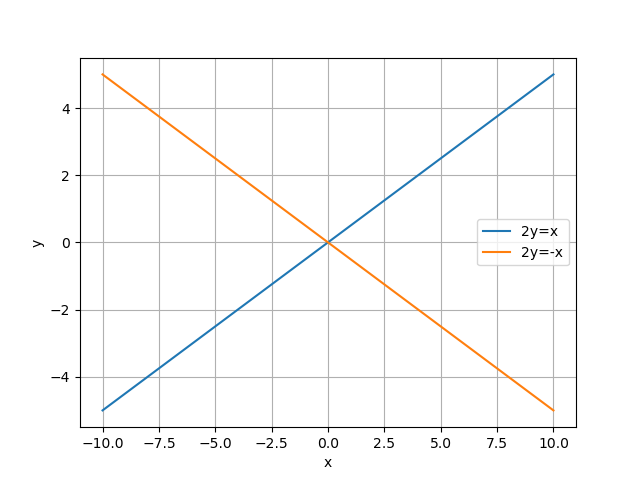
\includegraphics[width=\columnwidth]{Fig1_a5.png}
    \caption{straight lines after affine transformation passing through origin}
    \label{fig:1}
\end{figure}
This line will pass through origin,whose bisectors will be the $x-$axis and $y-$axis.The bisectors wil be of the form
\begin{align}
    \vec{y}^T\myvec{0&0.5\\0.5&0}\vec{y}=0\\
    \vec{y}^T\vec{K}\vec{y}=0\\
    \vec{K}=\myvec{0&0.5\\0.5&0}
\end{align}
\section{bisectors}
Taking the inverse of the affine transformation of the equation $xy=0$,will give the angle bisectors.
\begin{align}
    \brak{\vec{P}^{-1}\vec{x}-\vec{P}^{-1}c}^T\vec{K}\brak{\vec{P}^{-1}\vec{x}-\vec{P}^{-1}c}=0\\
    \vec{x}^T\vec{P}\vec{K}\vec{P}^T\vec{x}-2c^T\vec{P}\vec{K}\vec{P}^T\vec{x}+c^T\vec{P}\vec{K}\vec{P}^Tc=0
\end{align}
Substituting the values we get
\begin{align}
    \begin{multlined}
        \vec{x}^T\myvec{0.0238&0.5\\0.5&-0.0238}\vec{x}\\
        -\myvec{1.046&0.951}\vec{x}+1=0
    \end{multlined}\\
    \begin{multlined}
        0.0238x^2+xy-0.0238y^2\\
        -1.046x-0.951y+1=0
    \end{multlined}\\
    x^2+42xy-y^2-44x-40y+42=0
\end{align}
\begin{figure}[t]
    \centering
    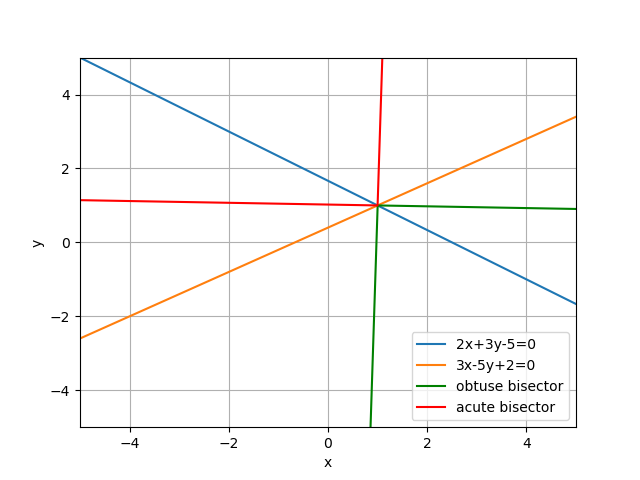
\includegraphics[width=\columnwidth]{Fig2_a5.png}
    \caption{Par of straight lines and their angular bisectors}
    \label{fig:my_label}
\end{figure}
\end{document}
